\chapter{Evaluation}

This chapter presents an evaluation of the constraints when applied to a number of open source systems. The evaluation was performed in two ways: first a comparison between SecArchUnit and static analysis tools used in industry, and then a standalone evaluation of the tool extension.

\section{Quantitative Results}
The quantitative evaluation aims to evaluate how well SecArchUnit can validate the 7 constraints and compare this to the performance of industrial-grade tools SonarQube and PMD. Due to the fact that not all constraints could be expressed in each of the three tools, the evaluation was divided into two stages.

In the first stage, constraints 1-5 were applied to each of the three test systems described in Section~\ref{sct:selected-systems}. These constraints were subsequently validated, not only in SecArchUnit, but also in SonarQube and PMD through definitions of custom rules. The results of this evaluation are presented in Table~\ref{tab:results_comparison}.

\newcolumntype{g}{>{\columncolor{RowColor}}c}
\newcolumntype{x}{>{\columncolor{RowColor}}l}
\begin{table}[h]
\begin{center}
\begin{tabular}{lxggggg}
\rowcolor{white}
\textbf{Project}           & \textbf{Tool}    & \textbf{TP} & \textbf{FP} & \textbf{FN} & \textbf{Precision} & \textbf{Recall} \\
\hline
\rowcolor{white}
\multirow[t]{3}{*}{ATMsim}    & SecArchUnit      & 19          & 1           & 0           & 1               & 0.95            \\
                           & SonarQube Plugin & 19          & 1           & 0           & 1               & 0.95            \\
                           \rowcolor{white}
                           & PMD Plugin       & 15          & 1           & 4           & 0.94               & 0.79            \\
\hline
\rowcolor{white}
\multirow[t]{3}{*}{JPetStore} & SecArchUnit      & 51          & 0           & 0           & 1                  & 1               \\
                           & SonarQube Plugin & 51          & 0           & 0           & 1                  & 1               \\
                           \rowcolor{white}
                           & PMD Plugin       & 47          & 0           & 4           & 1                  & 0.92            \\
\hline
\rowcolor{white}
\multirow[t]{3}{*}{ITrust}    & SecArchUnit      & 216         & 3           & 0           & 0.97               & 1               \\
                           & SonarQube Plugin & 216         & 0           & 0           & 1                  & 1               \\
                           \rowcolor{white}
                           & PMD Plugin       & 216         & 0           & 0           & 1                  & 1 \\
\hline
\end{tabular}
\end{center}
\caption{Results from validating constraints 1-5 using SecArchUnit, SonarQube and PMD.}
\label{tab:results_comparison}
\end{table}

In the second stage, constraints 6-7 were applied to iTrust and validated solely using SecArchUnit. The performance metrics resulting from this evaluation are presented in Table~\ref{tab:tool_extension}.

\begin{table}
\begin{center}
\begin{tabular}{lccccc}
\hline
\textbf{Constraint} & \textbf{TP} & \textbf{FP} & \textbf{FN} & \textbf{Precision} & \textbf{Recall} \\
\hline
6 & 24 & 0 & 0 & 1 & 1\\
\rowcolor{RowColor}
7 & 37 & 0 & 0 & 1 & 1\\
\hline
\end{tabular}
\end{center}
\caption{Results from validating the extension-based constraints on iTrust.}
\label{tab:tool_extension}
\end{table}

In both stages, the tools were evaluated according to the performance metrics. The true positives (TP) refer to violations of constraints that are reported by the tool and coincide with the ground truth. False positives (FP) are violations reported by the tool that are not included in the ground truth. False negatives (FN) are violations that exist in the ground truth but do not get reported by the tool. 

The number of violations of each constraint, according to our ground truth, can be seen in Figure~\ref{bar:frequency_violation_comparison}.

\begin{figure}
\centering
\captionsetup{justification=centering}

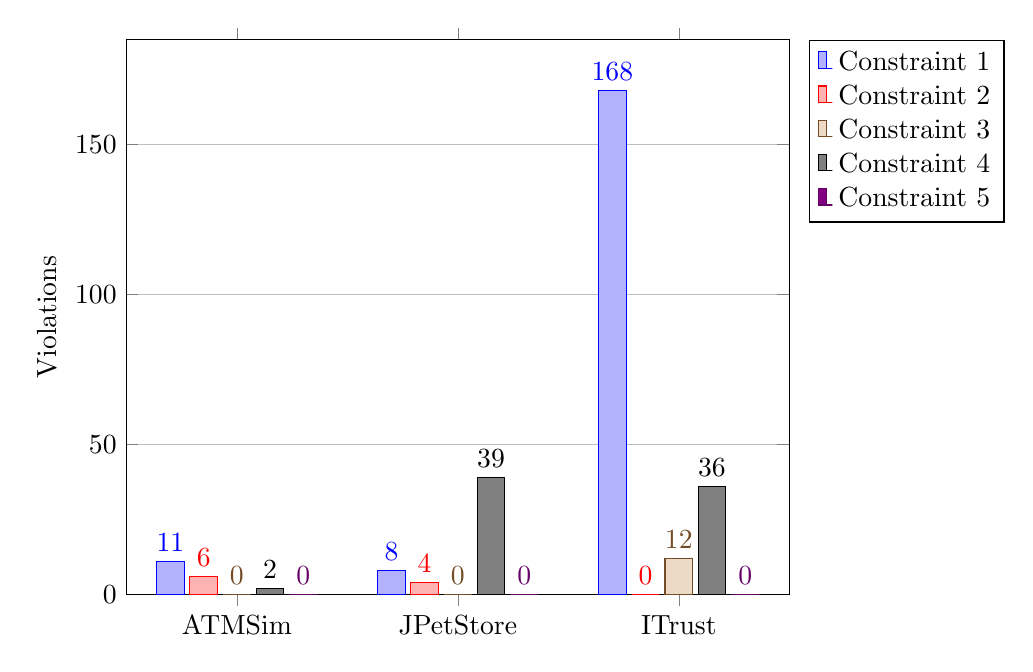
\begin{tikzpicture}
\begin{axis}[
    width=10cm,
    ybar,
    ymin = 0,
    ymajorgrids = true,
    enlarge x limits=0.25,
    xbar legend,
    legend pos=outer north east,
    ylabel={Violations},
    symbolic x coords={ATMSim,JPetStore,ITrust},
    %xlabel={System},
    xtick=data,
    nodes near coords,
    nodes near coords align={vertical},
    ]
%C1
\addplot coordinates {(ATMSim,11) (JPetStore,8) (ITrust,168)};
%C2
\addplot coordinates {(ATMSim,6) (JPetStore,4) (ITrust,0)};
%C3
\addplot coordinates {(ATMSim,0) (JPetStore,0) (ITrust,12)};
%C3
\addplot coordinates {(ATMSim,2) (JPetStore,39) (ITrust,36)};
%C3
\addplot coordinates {(ATMSim,0) (JPetStore,0) (ITrust,0)};
\legend{Constraint 1,Constraint 2,Constraint 3, Constraint 4, Constraint 5}
\end{axis}
\end{tikzpicture}

\caption{The constraint violations found in the ground truth of each system.}
\label{bar:frequency_violation_comparison}
\end{figure}




\section{Discussion of Quantitative Results}
Both in regards to precision, as well as recall, the tools performed equally. However, the causes of failure differed noticeably in cases where the results of the tools varied. The examples are described below:

\begin{itemize}
    \item In ATM simulator, the same false positive occurred in all three tools. This was in relation to constraint 3, where a subclass of the sending point contained a method call to the sender. Additionally, PMD had 4 false negatives which occurred because it was unable to determine the classes that these method calls targeted.
    \item In JPetStore, PMD reported 4 false negatives, again because it was unable to determine the target class of these method calls.
    \item In iTrust, a security service contained both an inner interface and an inner static class whose methods did not perform any security events. In both PMD and SonarQube, these methods were determined to be declared in the inner class by traversing the AST from the method to its first parent class or interface declaration. In comparison, ArchUnit considers the members of the inner class to be declared in both the inner and outer class. This improperly marks the inner methods as violating the constraint, resulting in 3 false positives.
\end{itemize}

As shown in Figure~\ref{bar:frequency_violation_comparison}, the tools were evaluated using imbalanced data. Constraint 1 accounted for a majority of all violations found throughout all three systems, while no system violated constraint 5. Additionally, iTrust was the only system to contain a violation of constraint 3. 

The system, iTrust, initially contained no violations of constraint 7. Therefore, violations were injected by systematically marking all identifier fields (e.g. \texttt{patientId}, \texttt{personnelId}) in the model and base-action packages as secrets. We chose to mark these identifiers because they were commonly sent to the logger as a way to describe the patient or personnel involved in a transaction. Hence, the 37 violations of constraint 7, as seen in Table~\ref{tab:tool_extension}, are artificially injected.

Moreover, iTrust is built with a mix of Java and Java Server Pages (JSP) files whereas ArchUnit can only analyze plain Java. The classes in the action package, from which the logger is called, are all instantiated in the JSP files outside the view of our analysis. As such, the types of information flow that are analyzed and included in the ground truth are rather rudimentary. Out of the 37 violations of constraint 7, 1 was found without recursion (direct access to secret field) and the remaining 36 were found using a single recursion step (access to getter method of a secret field).
% This is bad - we could just as well put the secret annotation on the getter and enforce the same constraint in SonarQube/PMD

\todo{Discuss examples of things that the tools won't catch}
% different levels of assets, i.e some fields are more sensitive than others



\section{Discussion of Qualitative Differences}
ArchUnit, SonarQube and PMD are all static analysis tools with support for evaluation of custom rules. However, they differ quite a bit in how their rules are defined and evaluated.

ArchUnit first builds a representation of the entirety of the analyzed system, which is then available during the evaluation of the rules. As shown throughout Chapter~\ref{ch:enforcing_constraints}, rules have direct access to information about incoming and outgoing accesses to all members, both within and between classes, making it convenient to specify intricate architectural constraints.

Regarding SonarQube and PMD, both of these tools evaluate rules against an Abstract Syntax Tree (AST) where the root node is the Java class currently being analyzed (see examples in Appendix~\ref{apx:sonarqube} and Appendix~\ref{apx:pmd}). As a consequence, a rule can only inspect one class at a time; it can audit outgoing accesses to other classes, but it does not know anything about incoming accesses to the current class and its members.
In a constraint where incoming accesses to a certain class need to be constrained, the rule can inspect all classes one by one and look for outgoing accesses to the concerned class. However, constraints that define more intricate control flows, such as allowing a given combination of incoming and outgoing accesses, are not enforceable in these tools.
% C4, third case, as example

Rule definitions - Abstract Syntax Trees (SonarQube \& PMD) vs higher-level abstraction (ArchUnit)

Analysis of accesses - expression chains, SonarQube vs PMD, PMD failures

Semantic information



\section{Threats to Validity}

\subsection{Construct Validity}

\subsection{Internal Validity}

\subsection{External Validity}